% Options for packages loaded elsewhere
\PassOptionsToPackage{unicode}{hyperref}
\PassOptionsToPackage{hyphens}{url}
%
\documentclass[
]{book}
\usepackage{amsmath,amssymb}
\usepackage{iftex}
\ifPDFTeX
  \usepackage[T1]{fontenc}
  \usepackage[utf8]{inputenc}
  \usepackage{textcomp} % provide euro and other symbols
\else % if luatex or xetex
  \usepackage{unicode-math} % this also loads fontspec
  \defaultfontfeatures{Scale=MatchLowercase}
  \defaultfontfeatures[\rmfamily]{Ligatures=TeX,Scale=1}
\fi
\usepackage{lmodern}
\ifPDFTeX\else
  % xetex/luatex font selection
\fi
% Use upquote if available, for straight quotes in verbatim environments
\IfFileExists{upquote.sty}{\usepackage{upquote}}{}
\IfFileExists{microtype.sty}{% use microtype if available
  \usepackage[]{microtype}
  \UseMicrotypeSet[protrusion]{basicmath} % disable protrusion for tt fonts
}{}
\makeatletter
\@ifundefined{KOMAClassName}{% if non-KOMA class
  \IfFileExists{parskip.sty}{%
    \usepackage{parskip}
  }{% else
    \setlength{\parindent}{0pt}
    \setlength{\parskip}{6pt plus 2pt minus 1pt}}
}{% if KOMA class
  \KOMAoptions{parskip=half}}
\makeatother
\usepackage{xcolor}
\usepackage{color}
\usepackage{fancyvrb}
\newcommand{\VerbBar}{|}
\newcommand{\VERB}{\Verb[commandchars=\\\{\}]}
\DefineVerbatimEnvironment{Highlighting}{Verbatim}{commandchars=\\\{\}}
% Add ',fontsize=\small' for more characters per line
\usepackage{framed}
\definecolor{shadecolor}{RGB}{248,248,248}
\newenvironment{Shaded}{\begin{snugshade}}{\end{snugshade}}
\newcommand{\AlertTok}[1]{\textcolor[rgb]{0.94,0.16,0.16}{#1}}
\newcommand{\AnnotationTok}[1]{\textcolor[rgb]{0.56,0.35,0.01}{\textbf{\textit{#1}}}}
\newcommand{\AttributeTok}[1]{\textcolor[rgb]{0.13,0.29,0.53}{#1}}
\newcommand{\BaseNTok}[1]{\textcolor[rgb]{0.00,0.00,0.81}{#1}}
\newcommand{\BuiltInTok}[1]{#1}
\newcommand{\CharTok}[1]{\textcolor[rgb]{0.31,0.60,0.02}{#1}}
\newcommand{\CommentTok}[1]{\textcolor[rgb]{0.56,0.35,0.01}{\textit{#1}}}
\newcommand{\CommentVarTok}[1]{\textcolor[rgb]{0.56,0.35,0.01}{\textbf{\textit{#1}}}}
\newcommand{\ConstantTok}[1]{\textcolor[rgb]{0.56,0.35,0.01}{#1}}
\newcommand{\ControlFlowTok}[1]{\textcolor[rgb]{0.13,0.29,0.53}{\textbf{#1}}}
\newcommand{\DataTypeTok}[1]{\textcolor[rgb]{0.13,0.29,0.53}{#1}}
\newcommand{\DecValTok}[1]{\textcolor[rgb]{0.00,0.00,0.81}{#1}}
\newcommand{\DocumentationTok}[1]{\textcolor[rgb]{0.56,0.35,0.01}{\textbf{\textit{#1}}}}
\newcommand{\ErrorTok}[1]{\textcolor[rgb]{0.64,0.00,0.00}{\textbf{#1}}}
\newcommand{\ExtensionTok}[1]{#1}
\newcommand{\FloatTok}[1]{\textcolor[rgb]{0.00,0.00,0.81}{#1}}
\newcommand{\FunctionTok}[1]{\textcolor[rgb]{0.13,0.29,0.53}{\textbf{#1}}}
\newcommand{\ImportTok}[1]{#1}
\newcommand{\InformationTok}[1]{\textcolor[rgb]{0.56,0.35,0.01}{\textbf{\textit{#1}}}}
\newcommand{\KeywordTok}[1]{\textcolor[rgb]{0.13,0.29,0.53}{\textbf{#1}}}
\newcommand{\NormalTok}[1]{#1}
\newcommand{\OperatorTok}[1]{\textcolor[rgb]{0.81,0.36,0.00}{\textbf{#1}}}
\newcommand{\OtherTok}[1]{\textcolor[rgb]{0.56,0.35,0.01}{#1}}
\newcommand{\PreprocessorTok}[1]{\textcolor[rgb]{0.56,0.35,0.01}{\textit{#1}}}
\newcommand{\RegionMarkerTok}[1]{#1}
\newcommand{\SpecialCharTok}[1]{\textcolor[rgb]{0.81,0.36,0.00}{\textbf{#1}}}
\newcommand{\SpecialStringTok}[1]{\textcolor[rgb]{0.31,0.60,0.02}{#1}}
\newcommand{\StringTok}[1]{\textcolor[rgb]{0.31,0.60,0.02}{#1}}
\newcommand{\VariableTok}[1]{\textcolor[rgb]{0.00,0.00,0.00}{#1}}
\newcommand{\VerbatimStringTok}[1]{\textcolor[rgb]{0.31,0.60,0.02}{#1}}
\newcommand{\WarningTok}[1]{\textcolor[rgb]{0.56,0.35,0.01}{\textbf{\textit{#1}}}}
\usepackage{longtable,booktabs,array}
\usepackage{calc} % for calculating minipage widths
% Correct order of tables after \paragraph or \subparagraph
\usepackage{etoolbox}
\makeatletter
\patchcmd\longtable{\par}{\if@noskipsec\mbox{}\fi\par}{}{}
\makeatother
% Allow footnotes in longtable head/foot
\IfFileExists{footnotehyper.sty}{\usepackage{footnotehyper}}{\usepackage{footnote}}
\makesavenoteenv{longtable}
\usepackage{graphicx}
\makeatletter
\def\maxwidth{\ifdim\Gin@nat@width>\linewidth\linewidth\else\Gin@nat@width\fi}
\def\maxheight{\ifdim\Gin@nat@height>\textheight\textheight\else\Gin@nat@height\fi}
\makeatother
% Scale images if necessary, so that they will not overflow the page
% margins by default, and it is still possible to overwrite the defaults
% using explicit options in \includegraphics[width, height, ...]{}
\setkeys{Gin}{width=\maxwidth,height=\maxheight,keepaspectratio}
% Set default figure placement to htbp
\makeatletter
\def\fps@figure{htbp}
\makeatother
\setlength{\emergencystretch}{3em} % prevent overfull lines
\providecommand{\tightlist}{%
  \setlength{\itemsep}{0pt}\setlength{\parskip}{0pt}}
\setcounter{secnumdepth}{5}
\usepackage{booktabs}
\ifLuaTeX
  \usepackage{selnolig}  % disable illegal ligatures
\fi
\usepackage[]{natbib}
\bibliographystyle{plainnat}
\IfFileExists{bookmark.sty}{\usepackage{bookmark}}{\usepackage{hyperref}}
\IfFileExists{xurl.sty}{\usepackage{xurl}}{} % add URL line breaks if available
\urlstyle{same}
\hypersetup{
  pdftitle={Laboratorio di agronomia di precisione},
  pdfauthor={Michele Croci},
  hidelinks,
  pdfcreator={LaTeX via pandoc}}

\title{Laboratorio di agronomia di precisione}
\author{Michele Croci}
\date{2024-07-11}

\usepackage{amsthm}
\newtheorem{theorem}{Theorem}[chapter]
\newtheorem{lemma}{Lemma}[chapter]
\newtheorem{corollary}{Corollary}[chapter]
\newtheorem{proposition}{Proposition}[chapter]
\newtheorem{conjecture}{Conjecture}[chapter]
\theoremstyle{definition}
\newtheorem{definition}{Definition}[chapter]
\theoremstyle{definition}
\newtheorem{example}{Example}[chapter]
\theoremstyle{definition}
\newtheorem{exercise}{Exercise}[chapter]
\theoremstyle{definition}
\newtheorem{hypothesis}{Hypothesis}[chapter]
\theoremstyle{remark}
\newtheorem*{remark}{Remark}
\newtheorem*{solution}{Solution}
\begin{document}
\maketitle

{
\setcounter{tocdepth}{1}
\tableofcontents
}
\hypertarget{prefazione}{%
\chapter{Prefazione}\label{prefazione}}

Benvenuti in un viaggio entusiasmante, dove scienza dei dati, statistica e agronomia si incontrano per andare verso il futuro dell'agricoltura. Questo corso introduttivo, progettato per studenti delle scienze agrarie, vi guiderà attraverso esercitazioni pratiche di analisi dati per affrontare le sfide quotidiane nel campo della ricerca e della produzione agricola.

L'\textbf{analisi dei dati} è diventata un pilastro fondamentale nella scienza moderna, aprendo nuove strade per soluzioni innovative, analisi approfondite e la garanzia di risultati riproducibili. Questo materiale, appositamente creato per studenti con poca o nessuna esperienza di analisi dati, vi accompagnerà passo dopo passo in questa avventura, partendo dai concetti base fino a raggiungere un livello di competenza che vi permetterà di esplorare, visualizzare, modellare e interpretare dati complessi.

R, il linguaggio scelto per questo percorso, è rinomato per la sua potenza nel campo della statistica e dell'analisi dati, nonché per la sua vasta adozione nella comunità scientifica. Grazie ad un ricco ecosistema di pacchetti e strumenti dedicati, R rende l'analisi dei dati accessibile e potente. Il codice presentato, affiancato da lezioni pratiche, vi familiarizzerà gradualmente con la sintassi di R, le sue funzioni principali e l'arte di trasformare dati grezzi in informazioni significative.

Il nostro obiettivo è quello di fornire un approccio equilibrato, combinando la complessità delle analisi con un uso oculato dei pacchetti. Sebbene i pacchetti offrano indubbi vantaggi in termini di efficienza e funzionalità, un eccessivo affidamento ad essi può ostacolare la comprensione dei concetti fondamentali dell'analisi dati. Attraverso l'utilizzo di dati reali provenienti da studi e progetti di ricerca, questo corso colma il divario tra teoria e pratica, offrendo esempi concreti e applicabili per consolidare le vostre competenze.

Nel corso della mia carriera, ho sperimentato in prima persona come l'analisi dei dati possa rivelare pattern nascosti, guidare decisioni informate e fornire una comprensione più profonda dei fenomeni agronomici. Spero sinceramente che possiate trovare in queste pagine non solo un percorso di apprendimento, ma anche un'autentica passione per l'analisi dei dati.

Benvenuti nel mondo dell'analisi dati applicata all'agronomia.

Buon divertimento!

\textbf{Michele Croci}\\
Assistant Professor in Agronomy \& Field Crops\\
Department of Sustainable Crop Production\\
Università Cattolica del Sacro Cuore

\textbf{License}

All the code in these book has been written entirely by the author unless noted otherwise. The entire material is available for free under the Creative Commons Attribution-NonCommercial-ShareAlike (\href{https://creativecommons.org/licenses/by-nc-sa/4.0/}{CC BY-NC-SA}) license

\hypertarget{coltivazioni-erbacee}{%
\chapter{Coltivazioni erbacee}\label{coltivazioni-erbacee}}

\hypertarget{introduzione}{%
\section{Introduzione}\label{introduzione}}

Il corso di coltivazioni erbacee mira a fornire una conoscenza approfondita delle tecniche colturali relative alle specie erbacee di pieno campo, evidenziandone l'importanza nel contesto agricolo italiano ed europeo. L'obiettivo principale è acquisire competenze nella gestione delle principali coltivazioni, tenendo conto non solo degli aspetti economici, sempre più influenzati dal mercato globale, ma anche dell'impatto ambientale delle scelte colturali.

Le \textbf{coltivazioni erbacee} sono estremamente diversificate e possono essere classificate in base a diversi criteri: - \textbf{Utilizzo finale}: cereali da olio, cereali da zucchero, ecc. - \textbf{Parte della pianta utilizzata:} fusto, radice, foglie, ecc. - \textbf{Tipo di coltivazione:} sarchiato, non sarchiato, ecc. - \textbf{Tradizionalità e innovazione:} colture tradizionali, alternative, o tradizionali con usi alternativi. - \textbf{Destinazione:} colture alimentari e non alimentari. - \textbf{Idoneità al set-aside:} colture coltivabili in regime di set-aside.

Gli \textbf{obiettivi primari} delle coltivazioni erbacee sono molteplici: - Massimizzazione delle rese - Ottimizzazione della qualità (ad esempio, contenuto proteico o oleico dei semi) - Massimizzazione del reddito Efficienza nell'uso dei fattori produttivi - Minimizzazione dell'impatto ambientale

L'agricoltura, nel corso della storia, ha permesso lo sviluppo della civiltà umana. Oggi, tuttavia, le scelte agricole devono considerare non solo la produttività, ma anche la sostenibilità ambientale. L'agricoltura moderna deve trovare un equilibrio tra la necessità di nutrire una popolazione in crescita e la salvaguardia dell'ambiente. L'inquinamento e il cambiamento climatico sono sfide cruciali che richiedono un approccio più sostenibile, come l'agricoltura integrata, che mira a ridurre l'impatto ambientale pur mantenendo rese soddisfacenti.

L'agricoltura, oltre a essere un settore economico fondamentale, svolge un ruolo cruciale nella produzione di cibo, nella salvaguardia del territorio e nella tutela dell'ambiente. Negli ultimi anni, l'importanza dell'agricoltura non alimentare e della bioeconomia è cresciuta notevolmente. Le piante non vengono più utilizzate solo per scopi alimentari, ma anche per la produzione di biogas, biocarburanti, medicine, tessuti e altri materiali.

Storicamente, l'agricoltura ha rappresentato il settore economico principale, impiegando una vasta percentuale della popolazione. Nei paesi sviluppati, questa percentuale è diminuita nel tempo, ma l'agricoltura rimane il settore primario, responsabile della produzione di cibo. A livello globale, l'agricoltura contribuisce in media per circa il 6\% al PIL, mentre nei paesi sviluppati questa percentuale scende all'1-2\%.

I cereali, in particolare \textbf{frumento e riso}, sono fondamentali nell'alimentazione umana, fornendo circa il 46\% delle calorie a livello globale. Le proteine animali contribuiscono per il 17\% all'apporto calorico, mentre cereali e prodotti animali forniscono rispettivamente il 42\% e il 39\% delle proteine nella dieta umana.

L'agricoltura contemporanea si trova ad affrontare la sfida di soddisfare i bisogni alimentari di una popolazione mondiale in crescita, che si prevede raggiungerà i 9 miliardi entro il 2050 e i 10 miliardi entro il 2100. Le sfide principali includono:

Aumentare la produzione di cibo: per far fronte alla crescita demografica e combattere la malnutrizione, che è un problema non solo di quantità ma anche di qualità della dieta. Produrre materie prime ed energia: sviluppare colture per usi non alimentari, come la produzione di biocarburanti e biomateriali. Limitare il degrado ambientale: adottare pratiche agricole sostenibili per ridurre l'impatto ambientale dell'agricoltura. Per aumentare la produzione agricola, sono state considerate diverse opzioni:

Espansione delle terre coltivate: questa opzione è stata scartata a causa del suo impatto negativo sull'ambiente, in particolare sulla deforestazione. Sfruttamento degli stock ittici: questa opzione presenta limitazioni a causa della capacità limitata degli ecosistemi marini. Aumento dei limiti di produzione: questa opzione è complessa e richiede un'attenta valutazione dei rischi ambientali e sanitari. Riduzione degli sprechi alimentari: questa opzione è considerata la più promettente e sostenibile, poiché una quantità significativa di cibo viene sprecata lungo la catena alimentare. La soluzione più efficace e sostenibile per aumentare la produzione agricola è il miglioramento dell'efficienza. Ciò significa ottimizzare l'uso delle risorse, come acqua, fertilizzanti e pesticidi, per ottenere rese più elevate senza aumentare l'impatto ambientale. La ricerca e lo sviluppo tecnologico svolgono un ruolo cruciale in questo processo, consentendo di sviluppare nuove varietà colturali, tecniche di coltivazione e sistemi di gestione più efficienti.

Lo studio di Chen et al.~(2011) sulla \textbf{gestione integrata suolo-coltura (ISSM)} per la sicurezza alimentare ha evidenziato l'importanza di un uso efficiente delle risorse per incrementare la produzione agricola e garantire la sicurezza alimentare. La ricerca sottolinea come l'adozione di nuove tecnologie e genotipi possa essere più complessa nei paesi più poveri (ad esempio, l'Africa subsahariana) rispetto a quelli in rapido sviluppo (ad esempio, la Cina).

In Cina, nonostante l'ampio utilizzo di OGM, fertilizzanti e prodotti fitosanitari, l'efficienza produttiva risulta spesso limitata. Ad esempio, un aumento del 50\% nell'uso di fertilizzanti ha portato ad un incremento della produzione di appena il 10\%. Per affrontare questa sfida, Chen e i suoi colleghi hanno sviluppato un modello che, basandosi sugli input agronomici, permette di calcolare la biomassa ottenibile. Il modello include un modulo per la simulazione del suolo e un altro per la simulazione della coltura, considerando anche l'accrescimento radicale delle piante nel bilancio idrico e dell'azoto. L'analisi climatica si basa su medie a lungo termine.

Attraverso simulazioni e confronti con le pratiche agricole effettive, i ricercatori hanno identificato combinazioni ottimali di input per massimizzare la produzione. In linea con i grafici di Tilman, lo studio conferma che, a parità di risorse, un utilizzo più efficiente di queste ultime può portare a notevoli miglioramenti nella produzione.

In particolare, la \textbf{gestione dell'azoto} emerge come un fattore cruciale. Il modello suggerisce non solo di bilanciare l'azoto in base agli input e agli output, ma anche di frazionare la sua applicazione, concentrando le dosi maggiori nelle fasi di rapido accrescimento della pianta. Il calcolo del bilancio dell'azoto deve considerare la coltura specifica, le asportazioni, l'area coltivata e le aspettative di produzione.

I risultati delle prove condotte in Cina dimostrano l'importanza di un uso efficiente dell'azoto. Ad esempio, una coltura di mais gestita con approcci ISSM (237 kg/ha di azoto e pratiche agricole avanzate) ha prodotto in media 13 t/ha, dimostrando una buona efficienza d'uso dell'azoto. Al contrario, una coltura fertilizzata con dosi eccessive di azoto (747 kg/ha), ma senza una gestione efficiente del sistema, ha prodotto solo 15,2 t/ha, evidenziando una scarsa efficienza d'uso.

In conclusione, lo studio di Chen et al.~(2011) sottolinea l'importanza di adottare un \textbf{approccio integrato} nella gestione del sistema suolo-coltura per massimizzare la produzione agricola e garantire la sicurezza alimentare. L'ottimizzazione dell'uso delle risorse, in particolare dell'azoto, e l'adozione di pratiche agricole efficienti sono fondamentali per raggiungere questo obiettivo.

\hypertarget{cereali}{%
\section{Cereali}\label{cereali}}

\hypertarget{frumento}{%
\subsection{Frumento}\label{frumento}}

Il frumento, sia esso tenero (Triticum aestivum) originario del Medio Oriente, sia duro (Triticum durum) proveniente dall'Africa centro-orientale, è la coltura più diffusa al mondo. Cina, India e Russia sono i principali produttori, ma Stati Uniti, Francia, Canada e Australia guidano le esportazioni. L'Italia, pur al 17° posto per la produzione totale, è leader insieme a Turchia e Canada nella coltivazione del grano duro, concentrata nelle regioni centro-meridionali, mentre quello tenero è coltivato principalmente al centro-nord.

Nonostante una superficie coltivata a frumento in diminuzione negli ultimi vent'anni (da 3,3 milioni di ettari nel 1984 agli attuali 2,35 milioni), con una produzione scesa da 10 a 8,64 milioni di tonnellate, il frumento resta una coltura fondamentale. Tuttavia, l'Italia non è autosufficiente e la dipendenza dalle importazioni è cresciuta nel tempo.

In sintesi, il frumento rappresenta una risorsa agricola cruciale a livello globale e nazionale, con l'Italia che gioca un ruolo di primo piano nella produzione di grano duro. Nonostante ciò, la sfida dell'autosufficienza rimane aperta e richiede attenzione costante.

\hypertarget{morfologia}{%
\subsubsection{Morfologia}\label{morfologia}}

\hypertarget{ciclo-vegetativo-e-riproduttivo}{%
\subsubsection{Ciclo vegetativo e riproduttivo}\label{ciclo-vegetativo-e-riproduttivo}}

\hypertarget{esigenze-ambientali}{%
\subsubsection{Esigenze ambientali}\label{esigenze-ambientali}}

\hypertarget{tecnica-colturale}{%
\subsubsection{Tecnica colturale}\label{tecnica-colturale}}

\hypertarget{avvicendamento}{%
\paragraph{Avvicendamento}\label{avvicendamento}}

\hypertarget{lavorazione-del-terreno}{%
\paragraph{Lavorazione del terreno}\label{lavorazione-del-terreno}}

\hypertarget{semina}{%
\paragraph{Semina}\label{semina}}

\hypertarget{epoca-di-semina}{%
\subparagraph{Epoca di semina}\label{epoca-di-semina}}

\hypertarget{scelta-del-seme-e-della-varietuxe0}{%
\subparagraph{Scelta del seme e della varietà}\label{scelta-del-seme-e-della-varietuxe0}}

\hypertarget{modalituxe0-e-densituxe0-di-semina}{%
\subparagraph{Modalità e densità di semina}\label{modalituxe0-e-densituxe0-di-semina}}

\hypertarget{concia-del-seme}{%
\subparagraph{Concia del seme}\label{concia-del-seme}}

\hypertarget{concimazione}{%
\paragraph{Concimazione}\label{concimazione}}

\hypertarget{concimazione-di-fondo-fosforo-e-potassio.}{%
\subparagraph{Concimazione di fondo (fosforo e potassio).}\label{concimazione-di-fondo-fosforo-e-potassio.}}

\hypertarget{concimazione-di-copertura-azoto.}{%
\subparagraph{Concimazione di copertura (azoto).}\label{concimazione-di-copertura-azoto.}}

\hypertarget{controllo-delle-erbe-infestanti}{%
\paragraph{Controllo delle erbe infestanti}\label{controllo-delle-erbe-infestanti}}

\hypertarget{diserbo-chimico}{%
\subparagraph{Diserbo chimico}\label{diserbo-chimico}}

\hypertarget{riso}{%
\subsection{Riso}\label{riso}}

\hypertarget{orzo}{%
\subsection{Orzo}\label{orzo}}

\hypertarget{erba-medica}{%
\subsection{Erba medica}\label{erba-medica}}

\hypertarget{mais}{%
\subsection{Mais}\label{mais}}

\hypertarget{fertilizzazione-azotata}{%
\section{Fertilizzazione azotata}\label{fertilizzazione-azotata}}

\hypertarget{campionamento-del-suolo}{%
\subsection{Campionamento del suolo}\label{campionamento-del-suolo}}

\hypertarget{epoca-di-campionamento}{%
\subsubsection{Epoca di campionamento}\label{epoca-di-campionamento}}

Deve essere scelta in funzione dello stato del terreno, che non dovrà essere né troppo secco né troppo umido. È opportuno intervenire in un momento sufficientemente lontano dagli interventi di lavorazione e di fertilizzazione; per le colture erbacee; l'epoca ottimale coincide con i giorni successivi alla raccolta, oppure almeno due mesi dopo l'ultimo apporto di concime.

\hypertarget{modalituxe0-di-campionamento}{%
\subsubsection{Modalità di campionamento}\label{modalituxe0-di-campionamento}}

Al fine di ottenere un campione rappresentativo, il prelevamento per le colture erbacee deve essere eseguito come segue:

\begin{itemize}
\item
  procedendo a zig zag nell'appezzamento, si devono individuare, a seconda dell'estensione, da 15 a 20 punti di prelievo di campioni elementari;
\item
  nei punti segnati, dopo aver asportato e allontanato i primi 5 cm al fine di eliminare la cotica erbosa e gli eventuali detriti superficiali presenti, si effettua il prelievo fino ad una profondità di 30 cm (0-30cm);
\item
  si sminuzza e si mescola accuratamente la terra proveniente dai prelievi eseguiti e, dopo aver rimosso ed allontanato pietre e materie organiche grossolane (radici, stoppie e residui
\end{itemize}

\href{https://www.youtube.com/watch?v=3_U9Z3fy0Ig}{Come fare un campionamento di suolo?}

\hypertarget{analisi-del-terreno}{%
\subsubsection{Analisi del terreno}\label{analisi-del-terreno}}

Le analisi fisico-chimiche costituiscono un importante strumento per una migliore conoscenza delle caratteristiche del terreno e bisogna quindi effettuare opportune analisi di laboratorio valutando i parametri e seguendo le metodologie più avanti specificate.

I parametri richiesti nell'analisi sono almeno:

\begin{itemize}
\item
  granulometria (tessitura),
\item
  pH in acqua,
\item
  sostanza organica (S.O., \%),
\item
  calcare totale e calcare attivo,
\item
  azoto totale (Ntotale, g/kg),
\item
  potassio scambiabile e
\item
  fosforo assimilabile.
\end{itemize}

In generale, si valuta che le analisi possano conservare la loro validità per un periodo massimo di 5 anni scaduto il quale occorre procedere, per la formulazione del piano di fertilizzazione, a nuove determinazioni.

\begin{longtable}[]{@{}
  >{\raggedright\arraybackslash}p{(\columnwidth - 8\tabcolsep) * \real{0.1944}}
  >{\raggedright\arraybackslash}p{(\columnwidth - 8\tabcolsep) * \real{0.1944}}
  >{\raggedright\arraybackslash}p{(\columnwidth - 8\tabcolsep) * \real{0.1944}}
  >{\raggedright\arraybackslash}p{(\columnwidth - 8\tabcolsep) * \real{0.1944}}
  >{\raggedright\arraybackslash}p{(\columnwidth - 8\tabcolsep) * \real{0.2222}}@{}}
\caption{Tabella x}\tabularnewline
\toprule\noalign{}
\begin{minipage}[b]{\linewidth}\raggedright
ID\_Suo
\end{minipage} & \begin{minipage}[b]{\linewidth}\raggedright
Descrizione
\end{minipage} & \begin{minipage}[b]{\linewidth}\raggedright
Classe
\end{minipage} & \begin{minipage}[b]{\linewidth}\raggedright
Raggruppamento
\end{minipage} & \begin{minipage}[b]{\linewidth}\raggedright
Gruppo
\end{minipage} \\
\midrule\noalign{}
\endfirsthead
\toprule\noalign{}
\begin{minipage}[b]{\linewidth}\raggedright
ID\_Suo
\end{minipage} & \begin{minipage}[b]{\linewidth}\raggedright
Descrizione
\end{minipage} & \begin{minipage}[b]{\linewidth}\raggedright
Classe
\end{minipage} & \begin{minipage}[b]{\linewidth}\raggedright
Raggruppamento
\end{minipage} & \begin{minipage}[b]{\linewidth}\raggedright
Gruppo
\end{minipage} \\
\midrule\noalign{}
\endhead
\bottomrule\noalign{}
\endlastfoot
1 & Sabbioso & Grossolana & Sabbiosi & tendenzialmente sabbioso \\
2 & Sabbioso Franco & Grossolana & Sabbiosi & tendenzialmente sabbioso \\
3 & Limoso & Media & Medio impasto & franco \\
4 & Franco Sabbioso & Media & Sabbiosi & tendenzialmente sabbioso \\
5 & Franco & Media & Medio impasto & franco \\
6 & Franco Limoso & Media & Medio impasto & franco \\
7 & Franco Sabbioso Argilloso & Media & Medio impasto & franco \\
8 & Franco Argilloso & Media & Medio impasto & franco \\
9 & Franco Limoso Argilloso & Media & Argillosi e limosi & tendenzialmente argilloso \\
10 & Argilloso Sabbioso & Fine & Argillosi e limosi & tendenzialmente argilloso \\
11 & Argilloso Limoso & Fine & Argillosi e limosi & tendenzialmente argilloso \\
12 & Argilloso & Fine & Argillosi e limosi & tendenzialmente argilloso \\
\end{longtable}

Per calcolare gli apporti di azoto da somministrare alla coltura, si applica la seguente relazione:

Concimazione azotata (N) =

fabbisogni colturali (A)

-- apporti derivanti dalla fertilità del suolo (B)

+ perdite per lisciviazione (C)

+ perdite per immobilizzazione e dispersione (D)

-- azoto da residui della coltura in precessione (E)

-- azoto da fertilizzazioni organiche effettuate negli anni precedenti (F)

-- apporti naturali (G).

\hypertarget{a.-fabbisogni-colturali-kgha-1}{%
\subsubsection{\texorpdfstring{A. Fabbisogni colturali (kg·ha\textsuperscript{-1})}{A. Fabbisogni colturali (kg·ha-1)}}\label{a.-fabbisogni-colturali-kgha-1}}

I fabbisogni colturali tengono conto della necessità di azoto della coltura, determinato sia sulla base degli assorbimenti colturali unitari che dalla produzione attesa, secondo quanto di seguito indicato:

\textbf{A = assorbimenti colturali unitari (\%) x produzione attesa (t ha\textsuperscript{-1}) x 10}

Gli assorbimenti unitari di riferimento sono riportati nell'allegato 6.Per le colture arboree da frutto il fabbisogno può essere anche stimato calcolando solo l'effettiva asportazione operata con la raccolta dei frutti (vedi allegato 6) a cui bisognerà però aggiungere una quota di azoto necessaria a sostenere la crescita annuale (quota di base, in kg, vedi Allegato 8).

\begin{longtable}[]{@{}
  >{\raggedright\arraybackslash}p{(\columnwidth - 8\tabcolsep) * \real{0.3514}}
  >{\raggedright\arraybackslash}p{(\columnwidth - 8\tabcolsep) * \real{0.1622}}
  >{\raggedright\arraybackslash}p{(\columnwidth - 8\tabcolsep) * \real{0.1622}}
  >{\raggedright\arraybackslash}p{(\columnwidth - 8\tabcolsep) * \real{0.1622}}
  >{\raggedright\arraybackslash}p{(\columnwidth - 8\tabcolsep) * \real{0.1622}}@{}}
\caption{Tabella 2. Coefficienti di assorbimento e asportazione delle colture per N, P2O5 e K2O in \% .}\tabularnewline
\toprule\noalign{}
\begin{minipage}[b]{\linewidth}\raggedright
Coltura
\end{minipage} & \begin{minipage}[b]{\linewidth}\raggedright
N
\end{minipage} & \begin{minipage}[b]{\linewidth}\raggedright
P2O5
\end{minipage} & \begin{minipage}[b]{\linewidth}\raggedright
K2O
\end{minipage} & \begin{minipage}[b]{\linewidth}\raggedright
Tipo Coeff. (**)
\end{minipage} \\
\midrule\noalign{}
\endfirsthead
\toprule\noalign{}
\begin{minipage}[b]{\linewidth}\raggedright
Coltura
\end{minipage} & \begin{minipage}[b]{\linewidth}\raggedright
N
\end{minipage} & \begin{minipage}[b]{\linewidth}\raggedright
P2O5
\end{minipage} & \begin{minipage}[b]{\linewidth}\raggedright
K2O
\end{minipage} & \begin{minipage}[b]{\linewidth}\raggedright
Tipo Coeff. (**)
\end{minipage} \\
\midrule\noalign{}
\endhead
\bottomrule\noalign{}
\endlastfoot
Barbababietola da zucchero (pianta intera) & 0.31 & 0.16 & 0.33 & asp \\
Grano duro (pianta intera) & 3.11 & 1.06 & 1.99 & ass \\
Grano duro (granella) & 2.42 & 0.85 & 0.59 & asp \\
Grano tenero FP/FPS (granella) & 2.41 & 0.78 & 0.50 & asp. \\
Grano tenero FP/FPS (pianta intera) & 2.96 & 0.98 & 1.87 & ass. \\
Grano tenero biscottiero (granella) & 2.08 & 0.98 & 0.61 & asp. \\
\end{longtable}

(*\emph{)} i coefficienti di asportazione sono quelli che considerano le quantità di elemento che escono dal campo con la raccolta della parte utile della pianta; mentre sono considerati di assorbimento quando comprendono anche le quantità di elemento che si localizzano nelle parti della pianta non raccolte e che rimangono in campo.

\begin{longtable}[]{@{}
  >{\raggedright\arraybackslash}p{(\columnwidth - 4\tabcolsep) * \real{0.5167}}
  >{\raggedright\arraybackslash}p{(\columnwidth - 4\tabcolsep) * \real{0.2000}}
  >{\raggedright\arraybackslash}p{(\columnwidth - 4\tabcolsep) * \real{0.2833}}@{}}
\caption{Tabella x. Scelta del ``coefficiente tempo'' per coltura, stagione di crescita e lunghezza del ciclo. I valori riportati in tabella sono da ritenersi indicativi perché possono variare in relazione all'effettiva lunghezza del ciclo e alla stagione di crescita}\tabularnewline
\toprule\noalign{}
\begin{minipage}[b]{\linewidth}\raggedright
Fase colturale/Ciclo
\end{minipage} & \begin{minipage}[b]{\linewidth}\raggedright
coefficiente
\end{minipage} & \begin{minipage}[b]{\linewidth}\raggedright
Esempio coltura
\end{minipage} \\
\midrule\noalign{}
\endfirsthead
\toprule\noalign{}
\begin{minipage}[b]{\linewidth}\raggedright
Fase colturale/Ciclo
\end{minipage} & \begin{minipage}[b]{\linewidth}\raggedright
coefficiente
\end{minipage} & \begin{minipage}[b]{\linewidth}\raggedright
Esempio coltura
\end{minipage} \\
\midrule\noalign{}
\endhead
\bottomrule\noalign{}
\endlastfoot
Prati pluriennali & 1.00 & erba medica 2° anno \\
a ciclo primaverile estivo \textgreater{} 130 gg & 0.75 & Mais classe 600 \\
a ciclo primaverile estivo da 100 a 130 gg & 0.67 & Mais classe 300 \\
a ciclo primaverile estivo da 70 a 100 gg & 0.50 & Melone \\
a ciclo primaverile estivo \textless{} 70 gg & 0.30 & Lattuga \\
a ciclo autunno vernino \textgreater{} 150 gg & 0.60 & Frumento \\
a ciclo autunno vernino \textless{} 150 gg & 0.50 & Pisello proteico \\
in secondo raccolto & 0.35 & Mais dopo loiessa \\
pluriennali in produzione & 1.00 & Asparago \\
\end{longtable}

\hypertarget{b.-apporti-di-azoto-derivanti-dalla-fertilituxe0-del-suolo-kgha-1}{%
\subsubsection{\texorpdfstring{B. Apporti di azoto derivanti dalla fertilità del suolo (kg·ha\textsuperscript{-1})}{B. Apporti di azoto derivanti dalla fertilità del suolo (kg·ha-1)}}\label{b.-apporti-di-azoto-derivanti-dalla-fertilituxe0-del-suolo-kgha-1}}

\hypertarget{esercizio-1}{%
\subsection{Esercizio 1}\label{esercizio-1}}

\hypertarget{esercizio-2}{%
\subsection{Esercizio 2}\label{esercizio-2}}

\hypertarget{irrigazione}{%
\section{Irrigazione}\label{irrigazione}}

\hypertarget{sistemi-di-irrigazione}{%
\subsection{Sistemi di irrigazione}\label{sistemi-di-irrigazione}}

\hypertarget{modelli-di-simulazione-delle-colture}{%
\chapter{Modelli di simulazione delle colture}\label{modelli-di-simulazione-delle-colture}}

Un modello, nella sua accezione più ampia, è una rappresentazione semplificata di un sistema ben delimitato nel mondo reale. In agricoltura, ad esempio, una coltura con i suoi organi e processi rappresenta un sistema complesso. Negli ultimi anni, i modelli di simulazione della crescita delle colture hanno acquisito un ruolo cruciale negli studi e nelle applicazioni agrometeorologiche, consentendo di analizzare il comportamento delle colture e la loro risposta all'ambiente circostante.

Una delle caratteristiche distintive di questi modelli è la loro capacità di fornire risultati validi anche in contesti agronomici, colturali e gestionali diversi da quelli in cui sono stati originariamente sviluppati. Questa versatilità ha elevato la modellistica a strumento complementare ideale alla sperimentazione tradizionale.

In generale, la costruzione di un modello consiste nell'identificazione di un insieme di equazioni matematiche che riproducano nel modo più accurato possibile il comportamento del sistema in esame.

\hypertarget{chapters-and-sub-chapters}{%
\section{Chapters and sub-chapters}\label{chapters-and-sub-chapters}}

There are two steps to cross-reference any heading:

\begin{enumerate}
\def\labelenumi{\arabic{enumi}.}
\tightlist
\item
  Label the heading: \texttt{\#\ Hello\ world\ \{\#nice-label\}}.

  \begin{itemize}
  \tightlist
  \item
    Leave the label off if you like the automated heading generated based on your heading title: for example, \texttt{\#\ Hello\ world} = \texttt{\#\ Hello\ world\ \{\#hello-world\}}.
  \item
    To label an un-numbered heading, use: \texttt{\#\ Hello\ world\ \{-\#nice-label\}} or \texttt{\{\#\ Hello\ world\ .unnumbered\}}.
  \end{itemize}
\item
  Next, reference the labeled heading anywhere in the text using \texttt{\textbackslash{}@ref(nice-label)}; for example, please see Chapter \ref{cross}.

  \begin{itemize}
  \tightlist
  \item
    If you prefer text as the link instead of a numbered reference use: \protect\hyperlink{cross}{any text you want can go here}.
  \end{itemize}
\end{enumerate}

\hypertarget{captioned-figures-and-tables}{%
\section{Captioned figures and tables}\label{captioned-figures-and-tables}}

Figures and tables \emph{with captions} can also be cross-referenced from elsewhere in your book using \texttt{\textbackslash{}@ref(fig:chunk-label)} and \texttt{\textbackslash{}@ref(tab:chunk-label)}, respectively.

See Figure \ref{fig:nice-fig}.

\begin{Shaded}
\begin{Highlighting}[]
\FunctionTok{par}\NormalTok{(}\AttributeTok{mar =} \FunctionTok{c}\NormalTok{(}\DecValTok{4}\NormalTok{, }\DecValTok{4}\NormalTok{, .}\DecValTok{1}\NormalTok{, .}\DecValTok{1}\NormalTok{))}
\FunctionTok{plot}\NormalTok{(pressure, }\AttributeTok{type =} \StringTok{\textquotesingle{}b\textquotesingle{}}\NormalTok{, }\AttributeTok{pch =} \DecValTok{19}\NormalTok{)}
\end{Highlighting}
\end{Shaded}

\begin{figure}

{\centering 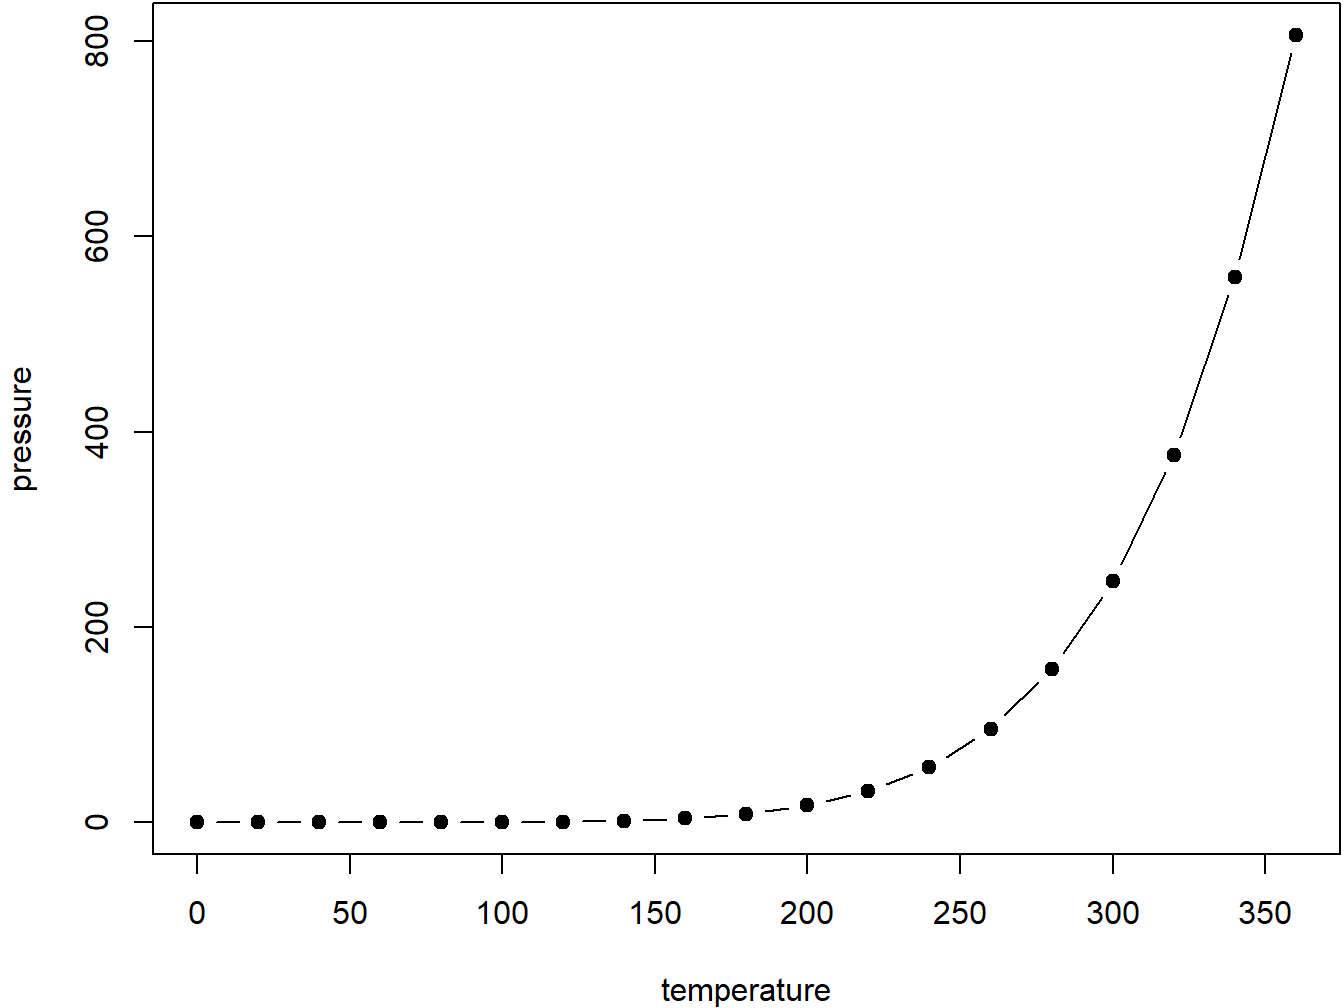
\includegraphics[width=0.8\linewidth]{_main_files/figure-latex/nice-fig-1} 

}

\caption{Here is a nice figure!}\label{fig:nice-fig}
\end{figure}

Don't miss Table \ref{tab:nice-tab}.

\begin{Shaded}
\begin{Highlighting}[]
\NormalTok{knitr}\SpecialCharTok{::}\FunctionTok{kable}\NormalTok{(}
  \FunctionTok{head}\NormalTok{(pressure, }\DecValTok{10}\NormalTok{), }\AttributeTok{caption =} \StringTok{\textquotesingle{}Here is a nice table!\textquotesingle{}}\NormalTok{,}
  \AttributeTok{booktabs =} \ConstantTok{TRUE}
\NormalTok{)}
\end{Highlighting}
\end{Shaded}

\begin{table}

\caption{\label{tab:nice-tab}Here is a nice table!}
\centering
\begin{tabular}[t]{rr}
\toprule
temperature & pressure\\
\midrule
0 & 0.0002\\
20 & 0.0012\\
40 & 0.0060\\
60 & 0.0300\\
80 & 0.0900\\
\addlinespace
100 & 0.2700\\
120 & 0.7500\\
140 & 1.8500\\
160 & 4.2000\\
180 & 8.8000\\
\bottomrule
\end{tabular}
\end{table}

\begin{Shaded}
\begin{Highlighting}[]
\FunctionTok{library}\NormalTok{(tidyverse)}
\end{Highlighting}
\end{Shaded}

\begin{verbatim}
## Warning: il pacchetto 'tidyverse' è stato creato con R versione 4.3.2
\end{verbatim}

\begin{verbatim}
## Warning: il pacchetto 'ggplot2' è stato creato con R versione 4.3.3
\end{verbatim}

\begin{verbatim}
## Warning: il pacchetto 'tidyr' è stato creato con R versione 4.3.3
\end{verbatim}

\begin{verbatim}
## Warning: il pacchetto 'readr' è stato creato con R versione 4.3.3
\end{verbatim}

\begin{verbatim}
## Warning: il pacchetto 'dplyr' è stato creato con R versione 4.3.3
\end{verbatim}

\begin{verbatim}
## Warning: il pacchetto 'stringr' è stato creato con R versione 4.3.2
\end{verbatim}

\begin{verbatim}
## Warning: il pacchetto 'lubridate' è stato creato con R versione 4.3.2
\end{verbatim}

\begin{verbatim}
## -- Attaching core tidyverse packages ------------------------ tidyverse 2.0.0 --
## v dplyr     1.1.4     v readr     2.1.5
## v forcats   1.0.0     v stringr   1.5.1
## v ggplot2   3.5.1     v tibble    3.2.1
## v lubridate 1.9.3     v tidyr     1.3.1
## v purrr     1.0.2     
## -- Conflicts ------------------------------------------ tidyverse_conflicts() --
## x dplyr::filter() masks stats::filter()
## x dplyr::lag()    masks stats::lag()
## i Use the conflicted package (<http://conflicted.r-lib.org/>) to force all conflicts to become errors
\end{verbatim}

\begin{Shaded}
\begin{Highlighting}[]
\CommentTok{\# Function to simulate soil water balance}
\NormalTok{soil\_water\_balance }\OtherTok{\textless{}{-}} \ControlFlowTok{function}\NormalTok{(soil\_params, rain, ET0, irrigation) \{}
  
  \CommentTok{\# Initialize soil water}
\NormalTok{  available\_water }\OtherTok{\textless{}{-}}\NormalTok{ soil\_params}\SpecialCharTok{$}\NormalTok{InitialAmountOfAvailableWater}
\NormalTok{  results }\OtherTok{\textless{}{-}} \FunctionTok{data.frame}\NormalTok{(}\AttributeTok{Day =} \DecValTok{1}\SpecialCharTok{:}\FunctionTok{length}\NormalTok{(rain))}
  
  \CommentTok{\# Loop through days}
  \ControlFlowTok{for}\NormalTok{ (day }\ControlFlowTok{in} \DecValTok{1}\SpecialCharTok{:}\FunctionTok{length}\NormalTok{(rain)) \{}
    
    \CommentTok{\# Calculate transpiration}
\NormalTok{    transpiration }\OtherTok{\textless{}{-}} \FunctionTok{min}\NormalTok{(}\FloatTok{0.096} \SpecialCharTok{*}\NormalTok{ available\_water, ET0[day]) }
    
    \CommentTok{\# Calculate surface runoff (SCS method)}
\NormalTok{    pot\_max\_ret }\OtherTok{\textless{}{-}}\NormalTok{ (}\DecValTok{25400} \SpecialCharTok{/}\NormalTok{ soil\_params}\SpecialCharTok{$}\NormalTok{RunoffCurveNumber) }\SpecialCharTok{{-}} \DecValTok{254}
\NormalTok{    init\_abs }\OtherTok{\textless{}{-}} \FloatTok{0.2} \SpecialCharTok{*}\NormalTok{ pot\_max\_ret}
\NormalTok{    surface\_runoff }\OtherTok{\textless{}{-}} \FunctionTok{ifelse}\NormalTok{(rain[day] }\SpecialCharTok{\textless{}=}\NormalTok{ init\_abs, }\DecValTok{0}\NormalTok{,}
\NormalTok{                             ((rain[day] }\SpecialCharTok{{-}}\NormalTok{ init\_abs)}\SpecialCharTok{\^{}}\DecValTok{2}\NormalTok{) }\SpecialCharTok{/}\NormalTok{ (rain[day] }\SpecialCharTok{{-}}\NormalTok{ init\_abs }\SpecialCharTok{+}\NormalTok{ pot\_max\_ret))}
    
    \CommentTok{\# Calculate deep drainage}
\NormalTok{    avail\_water\_before\_drain }\OtherTok{\textless{}{-}}\NormalTok{ available\_water }\SpecialCharTok{+}\NormalTok{ rain[day] }\SpecialCharTok{+}\NormalTok{ irrigation[day] }\SpecialCharTok{{-}}\NormalTok{ transpiration }\SpecialCharTok{{-}}\NormalTok{ surface\_runoff}
\NormalTok{    deep\_drainage }\OtherTok{\textless{}{-}} \FunctionTok{ifelse}\NormalTok{(soil\_params}\SpecialCharTok{$}\NormalTok{WaterHoldingCapacity }\SpecialCharTok{\textgreater{}=}\NormalTok{ (avail\_water\_before\_drain }\SpecialCharTok{/}\NormalTok{ soil\_params}\SpecialCharTok{$}\NormalTok{RootZoneDepth), }
                            \DecValTok{0}\NormalTok{, }
\NormalTok{                            soil\_params}\SpecialCharTok{$}\NormalTok{DrainageCoeff }\SpecialCharTok{*}\NormalTok{ soil\_params}\SpecialCharTok{$}\NormalTok{RootZoneDepth }\SpecialCharTok{*} 
\NormalTok{                              ((avail\_water\_before\_drain }\SpecialCharTok{/}\NormalTok{ soil\_params}\SpecialCharTok{$}\NormalTok{RootZoneDepth) }\SpecialCharTok{{-}}\NormalTok{ soil\_params}\SpecialCharTok{$}\NormalTok{WaterHoldingCapacity))}
    
    \CommentTok{\# Update available water}
\NormalTok{    available\_water }\OtherTok{\textless{}{-}}\NormalTok{ available\_water }\SpecialCharTok{+}\NormalTok{ rain[day] }\SpecialCharTok{+}\NormalTok{ irrigation[day] }\SpecialCharTok{{-}}\NormalTok{ transpiration }\SpecialCharTok{{-}}\NormalTok{ surface\_runoff }\SpecialCharTok{{-}}\NormalTok{ deep\_drainage}
    
    \CommentTok{\# Store results}
\NormalTok{    results}\SpecialCharTok{$}\NormalTok{Rain[day] }\OtherTok{\textless{}{-}}\NormalTok{ rain[day]}
\NormalTok{    results}\SpecialCharTok{$}\NormalTok{Deep\_drain[day] }\OtherTok{\textless{}{-}}\NormalTok{ deep\_drainage}
\NormalTok{    results}\SpecialCharTok{$}\NormalTok{Run\_off[day] }\OtherTok{\textless{}{-}}\NormalTok{ surface\_runoff}
\NormalTok{    results}\SpecialCharTok{$}\NormalTok{ET0[day] }\OtherTok{\textless{}{-}}\NormalTok{ ET0[day]}
\NormalTok{    results}\SpecialCharTok{$}\NormalTok{Transpi[day] }\OtherTok{\textless{}{-}}\NormalTok{ transpiration}
\NormalTok{    results}\SpecialCharTok{$}\NormalTok{Avlbl\_water[day] }\OtherTok{\textless{}{-}}\NormalTok{ available\_water}
\NormalTok{  \}}
  
  \FunctionTok{return}\NormalTok{(results)}
\NormalTok{\}}

\CommentTok{\# Example usage (replace with your actual data)}
\NormalTok{soil\_params }\OtherTok{\textless{}{-}} \FunctionTok{list}\NormalTok{(}
  \AttributeTok{InitialAmountOfAvailableWater =} \DecValTok{100}\NormalTok{,  }\CommentTok{\# mm}
  \AttributeTok{RunoffCurveNumber =} \DecValTok{85}\NormalTok{,}
  \AttributeTok{RootZoneDepth =} \DecValTok{1}\NormalTok{,                     }\CommentTok{\# m}
  \AttributeTok{DrainageCoeff =} \FloatTok{0.1}\NormalTok{,}
  \AttributeTok{WaterHoldingCapacity =} \FloatTok{0.2}            \CommentTok{\# mm/mm}
\NormalTok{)}

\CommentTok{\# Generate weather data for a year (365 days)}
\FunctionTok{set.seed}\NormalTok{(}\DecValTok{42}\NormalTok{)  }\CommentTok{\# For reproducibility}
\NormalTok{days }\OtherTok{\textless{}{-}} \DecValTok{1}\SpecialCharTok{:}\DecValTok{365}

\CommentTok{\# Rain: Simulate a seasonal pattern (higher in spring/fall)}
\NormalTok{rain }\OtherTok{\textless{}{-}} \DecValTok{20} \SpecialCharTok{*} \FunctionTok{abs}\NormalTok{(}\FunctionTok{sin}\NormalTok{(}\DecValTok{2} \SpecialCharTok{*}\NormalTok{ pi }\SpecialCharTok{*}\NormalTok{ days }\SpecialCharTok{/} \DecValTok{365}\NormalTok{)) }\SpecialCharTok{+} \FunctionTok{rnorm}\NormalTok{(}\DecValTok{365}\NormalTok{, }\DecValTok{0}\NormalTok{, }\DecValTok{5}\NormalTok{)  }\CommentTok{\# Seasonal + random noise}

\CommentTok{\# ET0: Simulate a seasonal pattern (higher in summer)}
\NormalTok{ET0 }\OtherTok{\textless{}{-}} \DecValTok{5} \SpecialCharTok{+} \DecValTok{3} \SpecialCharTok{*} \FunctionTok{abs}\NormalTok{(}\FunctionTok{sin}\NormalTok{(}\DecValTok{2} \SpecialCharTok{*}\NormalTok{ pi }\SpecialCharTok{*}\NormalTok{ (days }\SpecialCharTok{{-}} \DecValTok{90}\NormalTok{) }\SpecialCharTok{/} \DecValTok{365}\NormalTok{)) }

\CommentTok{\# Irrigation: Two scenarios}
\NormalTok{irrigation\_scenario1 }\OtherTok{\textless{}{-}} \FunctionTok{rep}\NormalTok{(}\DecValTok{0}\NormalTok{, }\DecValTok{365}\NormalTok{)  }\CommentTok{\# No irrigation}
\NormalTok{irrigation\_scenario2 }\OtherTok{\textless{}{-}} \FunctionTok{ifelse}\NormalTok{(days }\SpecialCharTok{\textgreater{}=} \DecValTok{150} \SpecialCharTok{\&}\NormalTok{ days }\SpecialCharTok{\textless{}=} \DecValTok{200}\NormalTok{, }\DecValTok{5}\NormalTok{, }\DecValTok{0}\NormalTok{)  }\CommentTok{\# 5 mm/day from June 1st to Sept 1st}

\CommentTok{\# Run the simulations for both scenarios}
\NormalTok{results\_scenario1 }\OtherTok{\textless{}{-}} \FunctionTok{soil\_water\_balance}\NormalTok{(soil\_params, rain, ET0, irrigation\_scenario1)}
\NormalTok{results\_scenario2 }\OtherTok{\textless{}{-}} \FunctionTok{soil\_water\_balance}\NormalTok{(soil\_params, rain, ET0, irrigation\_scenario2)}
\end{Highlighting}
\end{Shaded}

\begin{Shaded}
\begin{Highlighting}[]
\CommentTok{\# Reshape data for plotting}
\FunctionTok{library}\NormalTok{(tidyr)}
\NormalTok{results\_long\_scenario1 }\OtherTok{\textless{}{-}}\NormalTok{ results\_scenario1 }\SpecialCharTok{\%\textgreater{}\%}
  \FunctionTok{pivot\_longer}\NormalTok{(}\SpecialCharTok{{-}}\NormalTok{Day, }\AttributeTok{names\_to =} \StringTok{"Variable"}\NormalTok{, }\AttributeTok{values\_to =} \StringTok{"Value"}\NormalTok{) }\SpecialCharTok{\%\textgreater{}\%}
  \FunctionTok{mutate}\NormalTok{(}\AttributeTok{Scenario =} \StringTok{"No Irrigation"}\NormalTok{)}
\NormalTok{results\_long\_scenario2 }\OtherTok{\textless{}{-}}\NormalTok{ results\_scenario2 }\SpecialCharTok{\%\textgreater{}\%}
  \FunctionTok{pivot\_longer}\NormalTok{(}\SpecialCharTok{{-}}\NormalTok{Day, }\AttributeTok{names\_to =} \StringTok{"Variable"}\NormalTok{, }\AttributeTok{values\_to =} \StringTok{"Value"}\NormalTok{) }\SpecialCharTok{\%\textgreater{}\%}
  \FunctionTok{mutate}\NormalTok{(}\AttributeTok{Scenario =} \StringTok{"Irrigation"}\NormalTok{)}
\NormalTok{results\_long }\OtherTok{\textless{}{-}} \FunctionTok{rbind}\NormalTok{(results\_long\_scenario1, results\_long\_scenario2)}
\end{Highlighting}
\end{Shaded}

\begin{Shaded}
\begin{Highlighting}[]
\CommentTok{\# Plot the results using ggplot2}
\FunctionTok{library}\NormalTok{(ggplot2)}

\NormalTok{p }\OtherTok{\textless{}{-}} \FunctionTok{ggplot}\NormalTok{(results\_long, }\FunctionTok{aes}\NormalTok{(}\AttributeTok{x =}\NormalTok{ Day, }\AttributeTok{y =}\NormalTok{ Value, }\AttributeTok{color =}\NormalTok{ Scenario)) }\SpecialCharTok{+}
  \FunctionTok{geom\_line}\NormalTok{() }\SpecialCharTok{+}
  \FunctionTok{facet\_wrap}\NormalTok{(Variable}\SpecialCharTok{\textasciitilde{}}\NormalTok{., }\AttributeTok{scales =} \StringTok{"free\_y"}\NormalTok{) }\SpecialCharTok{+}  \CommentTok{\# Separate plots for each scenario}
  \FunctionTok{labs}\NormalTok{(}\AttributeTok{title =} \StringTok{"Soil Water Balance Simulation"}\NormalTok{, }\AttributeTok{x =} \StringTok{"Day of Year"}\NormalTok{, }\AttributeTok{y =} \StringTok{"Water (mm)"}\NormalTok{) }\SpecialCharTok{+}
  \FunctionTok{scale\_color\_manual}\NormalTok{(}\AttributeTok{values =} \FunctionTok{c}\NormalTok{(}\StringTok{"Irrigation"} \OtherTok{=} \StringTok{"blue"}\NormalTok{, }\StringTok{"No Irrigation"} \OtherTok{=} \StringTok{"orange"}\NormalTok{)) }\SpecialCharTok{+}
  \CommentTok{\# scale\_color\_manual(values = c("Rain" = "blue", "Deep\_drain" = "orange", }
    \CommentTok{\#                            "Run\_off" = "green", "ET0" = "red", }
    \CommentTok{\#                           "Transpi" = "purple", "Avlbl\_water" = "brown")) +}
  \FunctionTok{theme\_minimal}\NormalTok{()}

\FunctionTok{print}\NormalTok{(p)}
\end{Highlighting}
\end{Shaded}

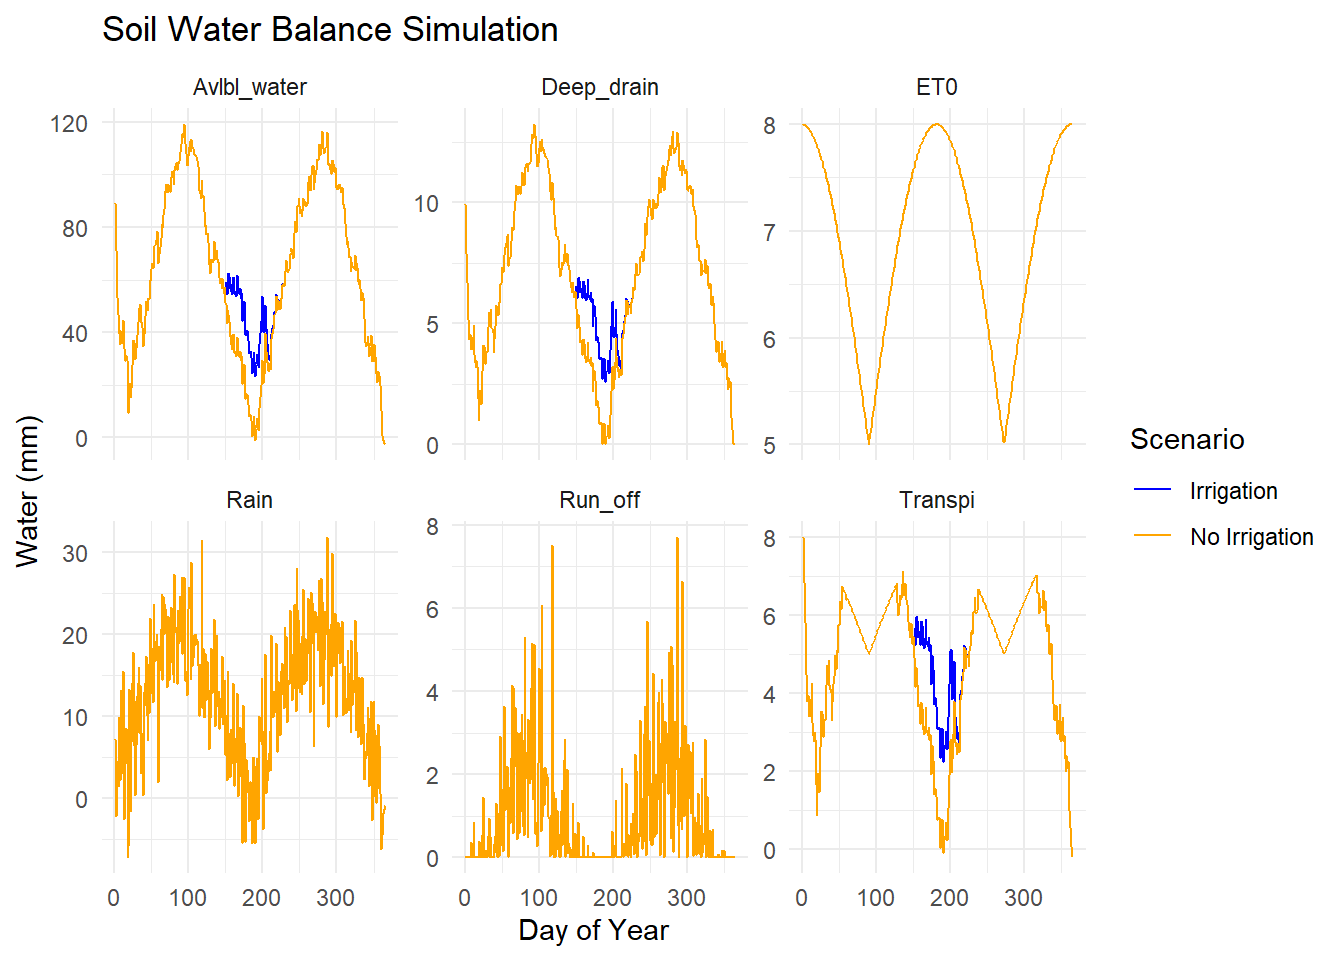
\includegraphics{_main_files/figure-latex/unnamed-chunk-3-1.pdf}

\hypertarget{concetti-base-di-programmazione}{%
\chapter{Concetti base di programmazione}\label{concetti-base-di-programmazione}}

\hypertarget{operazioni-di-base}{%
\section{Operazioni di base}\label{operazioni-di-base}}

\hypertarget{tipi-di-dati}{%
\section{Tipi di dati}\label{tipi-di-dati}}

\hypertarget{esercizi-generali}{%
\section{Esercizi generali}\label{esercizi-generali}}

You can add parts to organize one or more book chapters together. Parts can be inserted at the top of an .Rmd file, before the first-level chapter heading in that same file.

Add a numbered part: \texttt{\#\ (PART)\ Act\ one\ \{-\}} (followed by \texttt{\#\ A\ chapter})

Add an unnumbered part: \texttt{\#\ (PART\textbackslash{}*)\ Act\ one\ \{-\}} (followed by \texttt{\#\ A\ chapter})

Add an appendix as a special kind of un-numbered part: \texttt{\#\ (APPENDIX)\ Other\ stuff\ \{-\}} (followed by \texttt{\#\ A\ chapter}). Chapters in an appendix are prepended with letters instead of numbers.

\begin{Shaded}
\begin{Highlighting}[]
\ImportTok{import}\NormalTok{ numpy }\ImportTok{as}\NormalTok{ np}
\end{Highlighting}
\end{Shaded}

\hypertarget{analisi-dei-dati}{%
\chapter{Analisi dei dati}\label{analisi-dei-dati}}

\hypertarget{footnotes}{%
\section{Footnotes}\label{footnotes}}

Footnotes are put inside the square brackets after a caret \texttt{\^{}{[}{]}}. Like this one \footnote{This is a footnote.}.

\hypertarget{citations}{%
\section{Citations}\label{citations}}

Reference items in your bibliography file(s) using \texttt{@key}.

For example, we are using the \textbf{bookdown} package \citep{R-bookdown} (check out the last code chunk in index.Rmd to see how this citation key was added) in this sample book, which was built on top of R Markdown and \textbf{knitr} \citep{xie2015} (this citation was added manually in an external file book.bib). Note that the \texttt{.bib} files need to be listed in the index.Rmd with the YAML \texttt{bibliography} key.

The RStudio Visual Markdown Editor can also make it easier to insert citations: \url{https://rstudio.github.io/visual-markdown-editing/\#/citations}

\hypertarget{fondamenti-di-agricoltura-di-precisione}{%
\chapter{Fondamenti di agricoltura di precisione}\label{fondamenti-di-agricoltura-di-precisione}}

\hypertarget{geomatica}{%
\section{Geomatica}\label{geomatica}}

La geomatica può essere intesa come la scienza e l'insieme delle tecniche utilizzate per rispondere alle fondamentali domande connesse alla conoscenza qualitativa e quantitativa delle informazioni relative alla superficie terrestre (o a parti di essa) ed alle opere antropiche in essa presenti:

\begin{itemize}
\item
  Che cosa è (es. casa, strada, fiume, lago, particella, ecc\ldots)
\item
  Dove è (georeferenziazione)
\item
  Quanto è (misura ed elaborazione)
\end{itemize}

La geomatica viene applicata in tutte le discipline e le tecniche che si basano su dati spaziali georiferiti:

\begin{itemize}
\tightlist
\item
  Lo studio dell'ambiente e delle risorse naturali,
\item
  La pianificazione e gestione ambientale e territoriale,
\item
  La progettazione e realizzazione di opere di ingegneria,
\item
  la navigazione e più in generale i trasporti,
\item
  la geologia,
\item
  la geofisica,
\item
  la modellistica ambientale, climatica, meteorologica, agrometeo,
\item
  la gestione dei dati catastali,
\item
  l'\textbf{agricoltura}: 1. con applicazioni tradizionali (catasto di terreni, AGEA, SIAN,\ldots) e 2. con l'agricoltura di precisione
\end{itemize}

L'\textbf{anno zero} della geomatica è il \textbf{2004}, anno in cui Google compera Android e anche Google earth. In questo momento, operazioni che prima richiedevano software molto costosi (come ArcGIS, ArcInfo, ENVI, ERDAS) diventano gratuite (come Google Maps e QGIS). Prima di Google Maps, per avere delle mappe, si utilizzavano sistemi arcaici come Virgilio Mappe. Questi strumenti non erano neanche molto precisi.

Un'esempio di come utilizzare la geomatica in agricoltura, sta nel temutissimo catasto dei terreni ovvero un foglio in cui vengoni inserite le particelle (fabbricati più terreni di un tal signore) e i relativi comuni. L'AGEA (ovvero Agenzia Generale Erogazione in Agricoltura) invece unisce le ortofoto (foto presa da google earth) ai dati catastali per controllare la veridicità dell'informazione. AGEA opera attraverso il SIAN (Sistema Informativo Agricolo Nazionale), il Geoportale Nazionale

\hypertarget{agricoltura-di-precisione}{%
\section{Agricoltura di precisione}\label{agricoltura-di-precisione}}

E' l'applicazione di principi e tecnologie per la gestione della variabilità spaziale e temporale dei fattori connessi al processo produttivo agricolo, con lo scopo di migliorare la produzione e/o la sua qualità garantendo nel contempo migliori condizioni ambientali.

In altri termini: applicare il giusto input, nella giusta quantità, al momento giusto, nel posto giusto, nel modo giusto. Il focus è sulla variabilità spaziale, specialmente quella intraparcellare.

La chiave è nella georeferenziazione dei dati, ovvero dare un senso geografico (fornito di coordinate) al dato (pH, produttività, calcare,\ldots).

Il Sistema di Riferimento Globale per la georeferenziazione è WGS84 (che è l'ellissoide più famoso). I dati in forma di immagine o mappe di georeferenziazione si uniscono alle coordinate GPS del punto in cui ci troviamo tramite WGS84. Questo significa che dati indipendenti sono collegati tra di loro per via geografica.

\hypertarget{equations}{%
\section{Equations}\label{equations}}

Here is an equation.

\begin{equation} 
  f\left(k\right) = \binom{n}{k} p^k\left(1-p\right)^{n-k}
  \label{eq:binom}
\end{equation}

You may refer to using \texttt{\textbackslash{}@ref(eq:binom)}, like see Equation \eqref{eq:binom}.

\hypertarget{theorems-and-proofs}{%
\section{Theorems and proofs}\label{theorems-and-proofs}}

Labeled theorems can be referenced in text using \texttt{\textbackslash{}@ref(thm:tri)}, for example, check out this smart theorem \ref{thm:tri}.

\begin{theorem}
\protect\hypertarget{thm:tri}{}\label{thm:tri}For a right triangle, if \(c\) denotes the \emph{length} of the hypotenuse and \(a\) and \(b\) denote the lengths of the \textbf{other} two sides, we have \[a^2 + b^2 = c^2\]
\end{theorem}

Read more here \url{https://bookdown.org/yihui/bookdown/markdown-extensions-by-bookdown.html}.

\hypertarget{callout-blocks}{%
\section{Callout blocks}\label{callout-blocks}}

The R Markdown Cookbook provides more help on how to use custom blocks to design your own callouts: \url{https://bookdown.org/yihui/rmarkdown-cookbook/custom-blocks.html}

\hypertarget{telerilevamento-satellitare}{%
\chapter{Telerilevamento satellitare}\label{telerilevamento-satellitare}}

\hypertarget{definizioni-di-telerilevamento}{%
\section{Definizioni di telerilevamento}\label{definizioni-di-telerilevamento}}

Tre sono le più comuni definizioni che vengono date per il telerilevamento:

\begin{itemize}
\item
  Il telerilevamento è la scienza di acquisire, elaborare e interpretare immagini che registrano l'interazione tra l'energia elettromagnetica e la materia;
\item
  Il telerilevamento è la scienza o l'arte di ottenere informazioni circa un oggetto, un'area, o un fenomeno attraverso l'analisi di dati acquisiti per mezzo di un dispositivo che non è in contatto con l'oggetto, l'area o il fenomeno sotto esame.
\item
  Il telerilevamento è l'insieme della strumentazione, delle tecniche e dei metodi per osservare la superficie terrestre a distanza e per interpretare le immagini o i valori numerici ottenuti in modo da acquisire informazioni significative di oggetti particolari sulla Terra.
\end{itemize}

Comune alle tre definizioni è il fatto che i dati riguardanti le caratteristiche della superficie terrestre sono acquisiti con un dispositivo che non è in contatto con gli oggetti che si misurano. Il risultato è solitamente immagazzinato sotto forma di immagini. Le caratteristiche misurate dai sensori sono l'energia elettromagnetica emessa e riflessa dalla superficie terrestre. Questa energia riguarda alcune parti specifiche dello spettro elettromagnetico: di solito la luce visibile, ma anche l'infrarosso o le onde radio.

L'energia elettromagnetica generata da una opportuna sorgente (o dall'oggetto stesso) interagisce con l'oggetto osservato (fenomeni di riflessione, diffusione, assorbimento ecc) e di conseguenza si modifica. Tale radiazione si propaga e viene misurata e registrata da un sensore remoto. Analizzando e interpretando tali misure di campo elettromagnetico è possibile risalire alle proprietà di interesse dell'oggetto. Per particolari applicazioni geofisiche vengono usati altri tipi di campo, quali quello gravitazionale e magnetico della Terra e il campo di pressione (onde acustiche); basti pensare al sonar o semplicemente all'eco scandaglio per il sondaggio del fondale marino da imbarcazioni.

L'oggetto osservato può essere di varia natura; noi ci riferiremo a quei casi in cui esso è costituito dal nostro pianeta, la Terra, nelle sue diverse componenti (atmosfera, terre emerse, biosfera, oceani, ghiacci) che interagiscono tra loro attraverso processi chimico-fisici fondamentali per la conservazione della vita sul pianeta.

\hypertarget{energia-elettromagnetica-e-il-telerilevamento}{%
\section{Energia elettromagnetica e il telerilevamento}\label{energia-elettromagnetica-e-il-telerilevamento}}

\hypertarget{pages}{%
\section{404 pages}\label{pages}}

By default, users will be directed to a 404 page if they try to access a webpage that cannot be found. If you'd like to customize your 404 page instead of using the default, you may add either a \texttt{\_404.Rmd} or \texttt{\_404.md} file to your project root and use code and/or Markdown syntax.

\hypertarget{metadata-for-sharing}{%
\section{Metadata for sharing}\label{metadata-for-sharing}}

Bookdown HTML books will provide HTML metadata for social sharing on platforms like Twitter, Facebook, and LinkedIn, using information you provide in the \texttt{index.Rmd} YAML. To setup, set the \texttt{url} for your book and the path to your \texttt{cover-image} file. Your book's \texttt{title} and \texttt{description} are also used.

This \texttt{gitbook} uses the same social sharing data across all chapters in your book- all links shared will look the same.

Specify your book's source repository on GitHub using the \texttt{edit} key under the configuration options in the \texttt{\_output.yml} file, which allows users to suggest an edit by linking to a chapter's source file.

Read more about the features of this output format here:

\url{https://pkgs.rstudio.com/bookdown/reference/gitbook.html}

Or use:

\begin{Shaded}
\begin{Highlighting}[]
\NormalTok{?bookdown}\SpecialCharTok{::}\NormalTok{gitbook}
\end{Highlighting}
\end{Shaded}

\hypertarget{intelligenza-artificiale-in-agricoltura}{%
\chapter{Intelligenza artificiale in agricoltura}\label{intelligenza-artificiale-in-agricoltura}}

\hypertarget{supervised-machine-learning}{%
\section{Supervised machine learning}\label{supervised-machine-learning}}

\hypertarget{unsupervised-machine-learning}{%
\section{Unsupervised machine learning}\label{unsupervised-machine-learning}}

HTML books can be published online, see: \url{https://bookdown.org/yihui/bookdown/publishing.html}

\hypertarget{pages-1}{%
\section{404 pages}\label{pages-1}}

By default, users will be directed to a 404 page if they try to access a webpage that cannot be found. If you'd like to customize your 404 page instead of using the default, you may add either a \texttt{\_404.Rmd} or \texttt{\_404.md} file to your project root and use code and/or Markdown syntax.

\hypertarget{metadata-for-sharing-1}{%
\section{Metadata for sharing}\label{metadata-for-sharing-1}}

Bookdown HTML books will provide HTML metadata for social sharing on platforms like Twitter, Facebook, and LinkedIn, using information you provide in the \texttt{index.Rmd} YAML. To setup, set the \texttt{url} for your book and the path to your \texttt{cover-image} file. Your book's \texttt{title} and \texttt{description} are also used.

This \texttt{gitbook} uses the same social sharing data across all chapters in your book- all links shared will look the same.

Specify your book's source repository on GitHub using the \texttt{edit} key under the configuration options in the \texttt{\_output.yml} file, which allows users to suggest an edit by linking to a chapter's source file.

Read more about the features of this output format here:

\url{https://pkgs.rstudio.com/bookdown/reference/gitbook.html}

Or use:

\begin{Shaded}
\begin{Highlighting}[]
\NormalTok{?bookdown}\SpecialCharTok{::}\NormalTok{gitbook}
\end{Highlighting}
\end{Shaded}

\hypertarget{meccanizzazione-agraria}{%
\chapter{Meccanizzazione agraria}\label{meccanizzazione-agraria}}

\hypertarget{publishing}{%
\section{Publishing}\label{publishing}}

HTML books can be published online, see: \url{https://bookdown.org/yihui/bookdown/publishing.html}

\hypertarget{pages-2}{%
\section{404 pages}\label{pages-2}}

By default, users will be directed to a 404 page if they try to access a webpage that cannot be found. If you'd like to customize your 404 page instead of using the default, you may add either a \texttt{\_404.Rmd} or \texttt{\_404.md} file to your project root and use code and/or Markdown syntax.

\hypertarget{metadata-for-sharing-2}{%
\section{Metadata for sharing}\label{metadata-for-sharing-2}}

Bookdown HTML books will provide HTML metadata for social sharing on platforms like Twitter, Facebook, and LinkedIn, using information you provide in the \texttt{index.Rmd} YAML. To setup, set the \texttt{url} for your book and the path to your \texttt{cover-image} file. Your book's \texttt{title} and \texttt{description} are also used.

This \texttt{gitbook} uses the same social sharing data across all chapters in your book- all links shared will look the same.

Specify your book's source repository on GitHub using the \texttt{edit} key under the configuration options in the \texttt{\_output.yml} file, which allows users to suggest an edit by linking to a chapter's source file.

Read more about the features of this output format here:

\url{https://pkgs.rstudio.com/bookdown/reference/gitbook.html}

Or use:

\begin{Shaded}
\begin{Highlighting}[]
\NormalTok{?bookdown}\SpecialCharTok{::}\NormalTok{gitbook}
\end{Highlighting}
\end{Shaded}


  \bibliography{book.bib,packages.bib}

\end{document}
